%%%%%%%%%%%%%%%%%%%%%%%%%%%%%%%%%%%%%%%%%%%%%%%%%%%%%
\chapter{Introduction} \label{chap:intro}

\gls{hri} what it is and what it matters and why it is challenging

Robots will inhabit human spaces and need to interact with them in decent ways

%%%%%%%%%%%%%%%%%%%%%%%%%%%%%%%%%%%%%%%%%%%%%%%%%%%%%
\section{Scope}\label{sec:intro-scope}

\subsection{Frame}

\subsection{Environment} \label{sec:scope-social}
Robot interacting in an environment shared with humans / directly with humans
presence of a supervisor who can provide feedback/commands

\subsection{Type of interaction}

\begin{figure}[ht]
	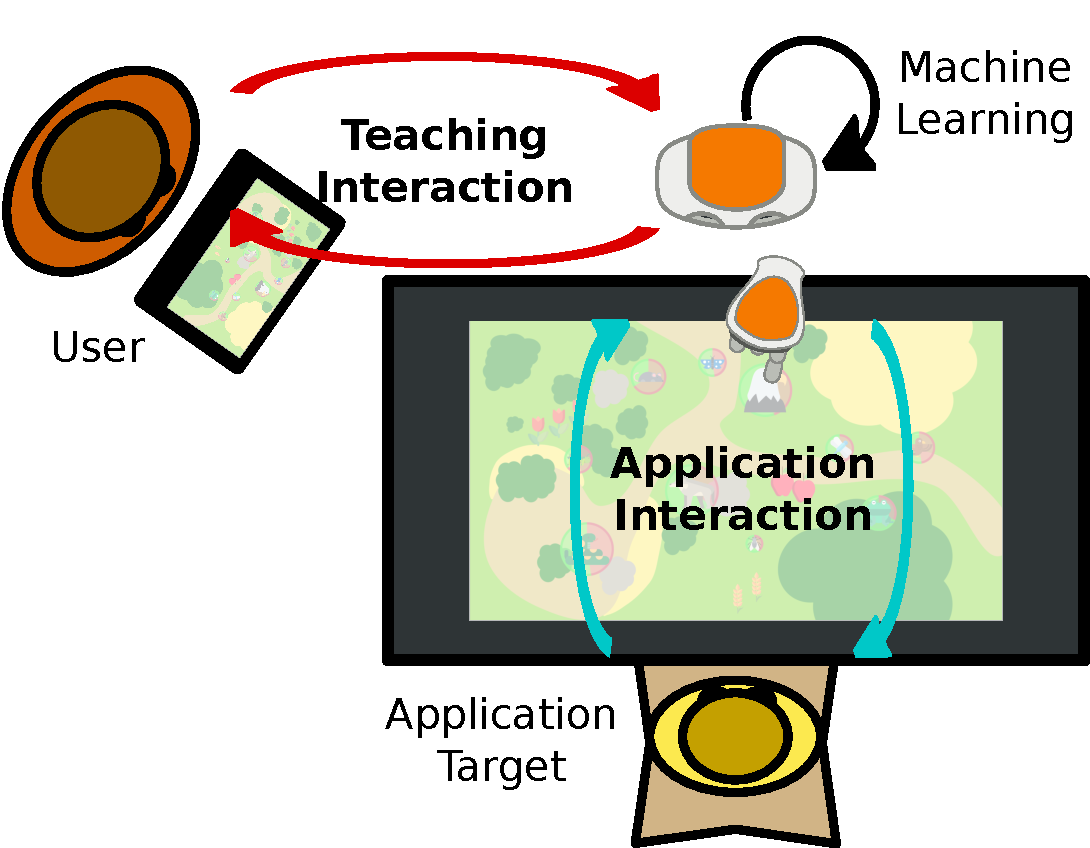
\includegraphics[width=.4\linewidth]{setup.pdf}
	\centering
	\caption{The setup used in the study: a child interacts with the robot tutor, with a large touchscreen sitting between them displaying the learning activity; a human teacher provides guidance to the robot through a tablet and monitors the robot's learning.}
	\label{fig:setup}
\end{figure}

\subsection{Algorithms}


%%%%%%%%%%%%%%%%%%%%%%%%%%%%%%%%%%%%%%%%%%%%%%%%%%%%%
\section{The Thesis}\label{sec:intro-thesis}
The main thesis that this document seeks to put forward is as below.

A robot can learn how to interact meaningfully with humans by receiving teaching
content from a human supervisor which leads to an efficient, safe and
low human-workload interaction policy.
%One sentence to describe the take home/conclusion

Additional research questions have been explored during the progress of this
work and are introduced here.

\begin{itemize}
    \item \textbf{Does adding a learning component to a supervised robot can reduce the human-workload of the supervisor?}\\
    
        \gls{woz} is an approach widely used in \gls{hri} \citep{riek2012wizard}, whereby a human teleoperates a robot to have it interact with other humans. However, this method applies a high workload on the operator and is not scalable. Using \gls{ml} to learn from this operator online might decrease the operator's workload without decreasing the quality of the robot behaviour.
    
    \item \textbf{How control of a teacher over the robot's action impacts the robot's learning?} 
    
	    In the context of \gls{iml}, a human can provide inputs to an agent to speed up the learning. Other \gls{iml} \citep{thomaz2008teachable,knox2009interactively} focus on feedback from the human with limited or no control over the agent's actions. However increase the control should speed up the learning and reduce the number of errors made by the robot.

    \item \textbf{How could a human teach a robot how to interact with other humans?}

	 \gls{sparc} has been designed to allow non-experts in \gls{ml} to teach agents how to interact while interacting. Human-robot interactions provide a perfect test for this approach: using a human to teach a robot how to behave in this complex and non-deterministic environment.


\end{itemize}

%%%%%%%%%%%%%%%%%%%%%%%%%%%%%%%%%%%%%%%%%%%%%%%%%%%%%
\section{Approach and Experimentation}\label{sec:intro-exps}

%%%%%%%%%%%%%%%%%%%%%%%%%%%%%%%%%%%%%%%%%%%%%%%%%%%%%
\section{Key Concepts}\label{sec:intro-concepts}

%%%%%%%%%%%%%%%%%%%%%%%%%%%%%%%%%%%%%%%%%%%%%%%%%%%%%
\section{Challenges}

%%%%%%%%%%%%%%%%%%%%%%%%%%%%%%%%%%%%%%%%%%%%%%%%%%%%%
\section{Contributions}\label{sec:intro-contr}

\begin{itemize}
	\item Something 
\end{itemize}

%%%%%%%%%%%%%%%%%%%%%%%%%%%%%%%%%%%%%%%%%%%%%%%%%%%%%
\section{Structure}\label{sec:intro-struct}
The structure of this thesis is outlined below to provide an overview of the content and context for each chapter. A summary of key experimental findings are included at the start of each relevant chapter for ease of reference. 

\begin{itemize}
\item This chapter provided an introduction to the general field of this research (robot tutors for children), the research questions including the central \textit{thesis}, scope, and contributions of the work presented in later chapters.  

\item Chapter~\ref{chap:background} 

%\item Chapter \ref{chap:method}

%\item Chapter \ref{chap:maindisc} draws on the experimental work from previous chapters, alongside the context supplied by related work, to form a discussion about the broader context and findings of the thesis. Limitations of the work conducted here are outlined, leading to suggestions for future directions of research.

\item Chapter~\ref{chap:conclusion} concludes the thesis with a summary of the main contributions.

\end{itemize}
